\documentclass[11pt]{article}
\usepackage{graphicx}
\usepackage{amsmath}
\usepackage{amssymb}
\usepackage{color}
\usepackage{subcaption}
\usepackage{listings}
\font\reallybigtenb=cmb10 scaled\magstep3
\parindent=0pt
\parskip=8.0pt
\baselineskip=12pt
\oddsidemargin=-0.5cm
\textwidth=17cm
\topmargin=-1.4cm
\textheight=23.0cm

\definecolor{codegreen}{rgb}{0,0.6,0}
\definecolor{codegray}{rgb}{0.5,0.5,0.5}
\definecolor{codepurple}{rgb}{0.58,0,0.82}
\definecolor{backcolour}{rgb}{0.95,0.95,0.92}
\lstdefinestyle{mystyle}{
    backgroundcolor=\color{backcolour},
    commentstyle=\color{codegreen},
    keywordstyle=\color{magenta},
    numberstyle=\tiny\color{codegray},
    stringstyle=\color{codepurple},
    basicstyle=\ttfamily\footnotesize,
    breakatwhitespace=false,
    breaklines=true,
    captionpos=b,
    keepspaces=true,
    numbers=none,
    numbersep=5pt,
    showspaces=false,
    showstringspaces=false,
    showtabs=false,
    tabsize=2}
\lstset{style=mystyle}

\begin{document}
    \begin{center}
        {\reallybigtenb{MTH1003}}

        {\reallybigtenb{Model of Competition Between Species}}

        \vspace{1mm}
        Group 24:

        Aiden Burrell-Saward, Abby Pallot, Maddie Bell, Faith Muga, Jonas Brown, Nirmay Patel

    \end{center}
    \begin{center}
    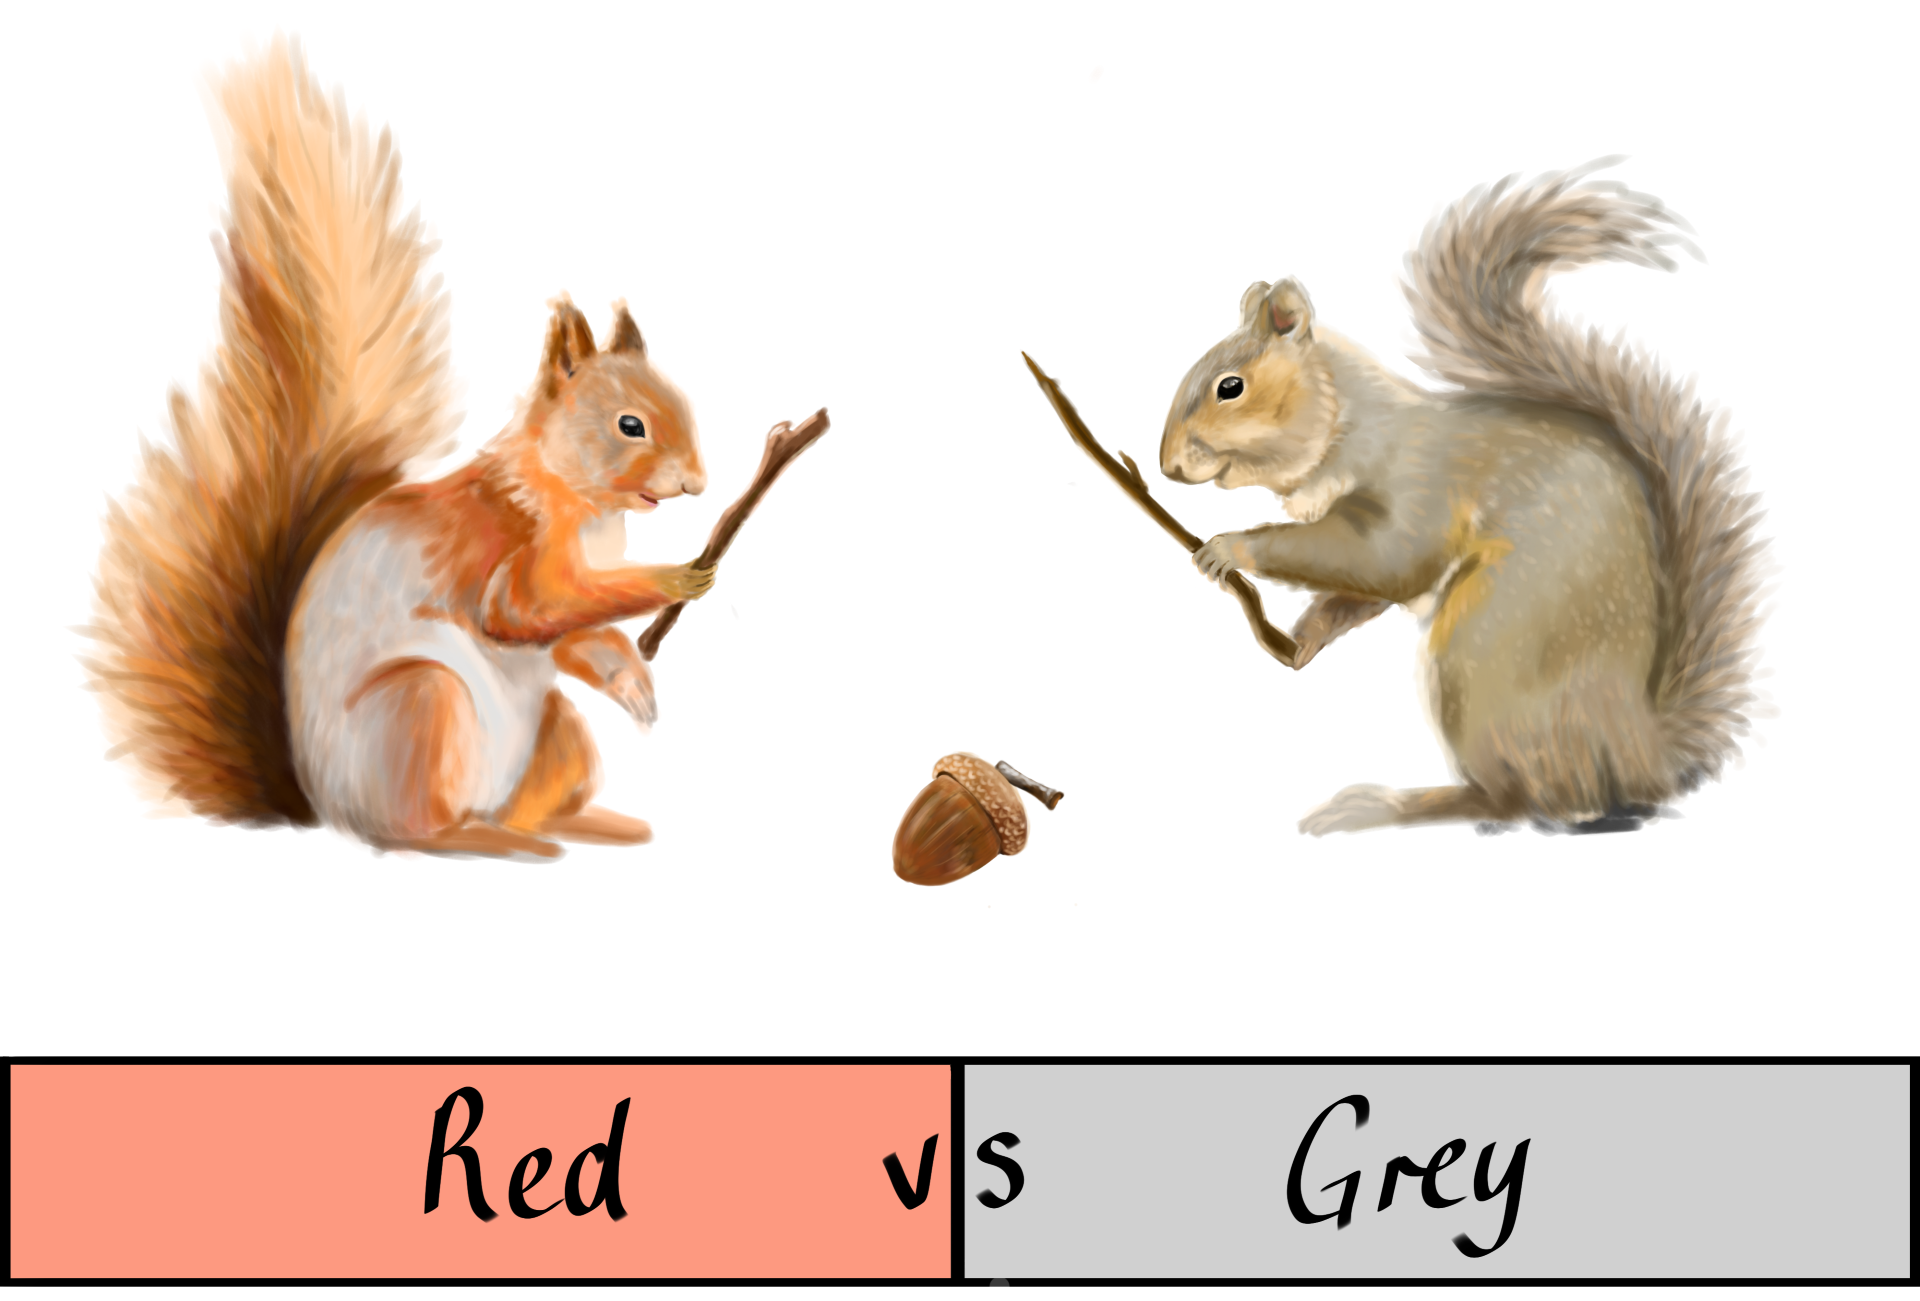
\includegraphics[scale = 1.1]{./images/squirrel_IMG_0256}
    \end{center}
    \subsection*{Introduction:}

    We have been tasked with using various mathematical modelling methods in order to study the Lotka-Volterra model of competition between two species of squirrel.

    \vspace{2mm}

    \subsection*{Equilibrium Points}

    In question 1, we are asked to find the equilibrium points of the system:
    \begin{equation}
        \dot{r} = r(1 - g), \qquad \dot{g} = g(2 - r).
    \end{equation}
    We found these points by setting $\dot{r}=0,\dot{g}=0$ and then finding the subsequent r and g values which satisfy the equality.
    \[\dot{r} = r(1 - g) = r - rg = 0 \quad \therefore \quad r = 0 \quad g = 1\]
    \[\dot{g} = g(2 - r) = 2g - rg = 0 \quad \therefore \quad r = 2 \quad g = 0\]

    By substituting these values of r and g back into both $\dot{r}=0$ and $\dot{g}=0$, we obtain the equilibrium points that are: $(0,0)$ and $(2,1)$. To classify these equilibrium points, a Jacobian matrix ($M$) was formed where $1-g=\ddot{r}$,$-r=\frac{d}{dg}$($\dot{r}$), $-g=\frac{d}{dr}$($\dot{r}$) and $2-r=\ddot{g}$. We then proceeded to substitute each equilibrium point into $M$ and find the corresponding eigenvalues:

    \[M = \begin{pmatrix} 1 - g & - r \\ - g & 2 - r
        \end{pmatrix}\]
    \[\therefore det(M-\lambda I) = 0 = (1-g - \lambda)(2 - r - \lambda) - rg\\\]
    \[
        \lambda = \frac{(3-r-g)\pm\sqrt{(3-r-g)^2-4(2-2g-r)}}{2}
    \]
    So for $(0,0)$:
    \[
        \lambda = \frac{3\pm\sqrt{1}}{2}
    \]
    \[
        \therefore \lambda = 1, \lambda = 2
    \]

    Both lambda values are real and positive which means that $(0,0)$ is an improper unstable node.

    Then for $(2,1)$:
    \[
        \lambda = \frac{\pm\sqrt{8}}{2}
    \]
    \[
        \therefore \lambda = \sqrt{2}, \lambda = -\sqrt{2}
    \]

    Both lambda values are real but one value is negative and the other is positive. This means that $(2,1)$ is a saddle point.

    \vspace{2mm}

   Later in the question, we are asked to show that the below quantity is conserved in this system:
    \[
        C(r,g) = \frac{r^2}{g}\exp{(g-r)}
    \]


    As $\dot{r}$ and $\dot{g}$ are functions of $t$, $\dot{r}$ and $\dot{g}$ are not linear. Therefore, to show conservation, we need to linearise this system. To do this, we start off by separating the variables; this allows us to integrate the system and provide the required result.


    \[
        \frac{dg}{dr} = \frac{\dot{g}}{\dot{r}} =  \frac{g(2-r)}{r(1-g)}
    \]
    \[
        \therefore \frac{1-g}{g}\frac{dg}{dr} = \frac{2-r}{r}
    \]
    By integrating with respect to $r$, we get:
    \[
        \int\frac{1-g}{g}dr\frac{dg}{dr} = \int\frac{2-r}{r}dr
    \]
    \[
        \therefore ln(g) - g = 2ln(r) + d\\
    \]
    \[
        \therefore e^{ln(g)-g} = e^{2ln(r)-r+d}
    \]
     \[
        1 = e^{2ln(r)-r-ln(g)+g+d}
    \]
    \[
        \therefore  C(r,g)= e^{-d} = e^{2ln(r)-ln(g)}e^{g-r}
    \]
    Thus, we have:
    \[
        C(r,g) = \frac{r^2}{g}e^{g-r}
    \]
    Therefore, this constant $C$ is conserved for this system.

    \vspace{2mm}


    \subsection*{Numerical simulation and testing}

    To graph this Lotka-Volterra model, we used a forward Euler timestepping scheme with initial conditions of $(r(0),g(0)) = (0.5,0.0116)$ within the boundary $t \epsilon [0,6]$, and a timestep $\Delta t=0.1$. We then graphed $r$ and $g$ against time, as well as the value of $C(r,g)$, which we previously showed to be constant mathematically. As we know $C(r,g)$ should be constant, we can use this to gauge how accurate our model is.
    \begin{figure}
        \begin{subfigure}{0.5\textwidth}
            \centering
            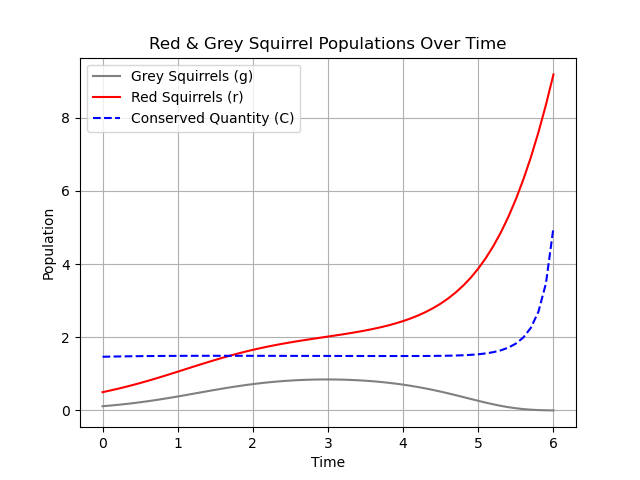
\includegraphics[scale = 0.45]{./images/Q2fig1}
            \caption{$\Delta t=0.1$}
            \label{fig:randg1}
        \end{subfigure}
        \begin{subfigure}{0.5\textwidth}
            \centering
            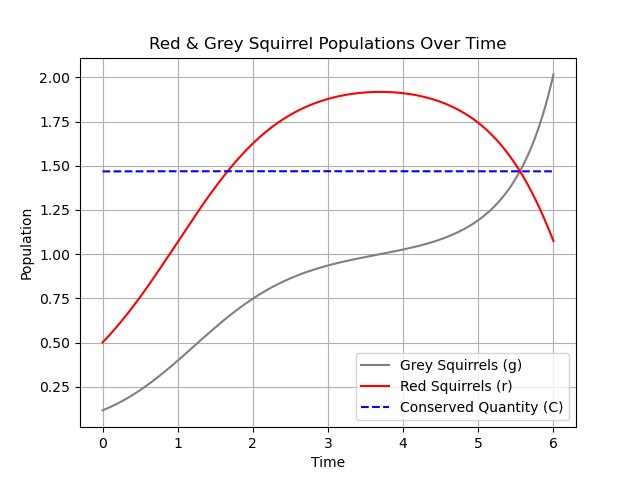
\includegraphics[scale = 0.45]{./images/Q2fig2}
            \caption{$\Delta t=0.003125$}
            \label{fig:randg2}
        \end{subfigure}
    \label{fig:randg}
    \caption{Population of red and grey squirrels using $(1)$ and different $\Delta t$}
    \end{figure}

    As can be seen in Figure \ref{fig:randg1}, When using such a large timestep, this Euler scheme is not a good fit for the model, demonstrated by the fact that the quantity $C(r,g)$ is not conserved. However, we can make our model a better fit by finding a $\Delta t$ ($\Delta t_{0}$) value small enough to ensure a small relative change in $C(r,g)$. We found $\Delta t_{0}=0.003125$ to produce a much more accurate model, with very little deviation in the quantity $C(r,g)$, as seen in Figure \ref{fig:randg2}.
    \begin{figure}
        \centering
        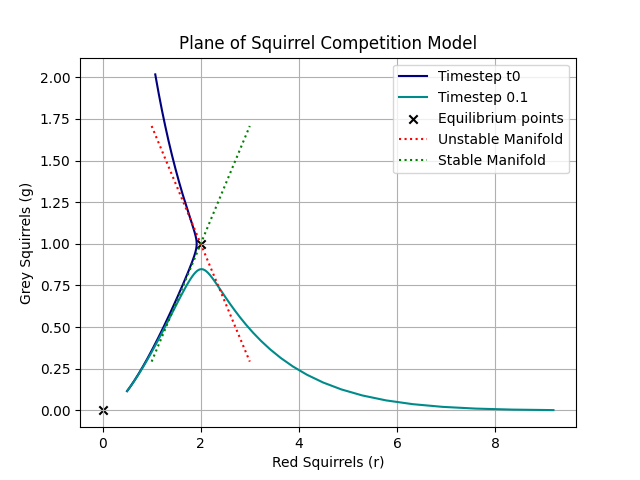
\includegraphics[scale = 0.5]{./images/plane-of-squirrel-competition-model}
        \caption{Comparison of the model with $\Delta t=0.003125$ and $\Delta t=0.1$}
        \label{fig:timesteps}
    \end{figure}
    In Figure \ref{fig:timesteps}, the difference in the two Euler schemes is clear, as they take completely different paths, going on either side of the saddle point, in the same direction as its unstable manifolds.

    \subsection*{Stable and unstable manifolds}
   In this question, we are asked to determine the directions of the stable and unstable manifolds close to the saddle by using using linear stability theory.

   We have a saddle point $(2,1)$ which we obtained in question 1. To determine the directions of the stable and unstable manifolds, we again use the Jacobian matrix we previously formed. We substitute the values of this point into $M$ to produce:

   \[
        M = \begin{pmatrix} 1 - g - \lambda  & - r \\ - g & 2 - r - \lambda
        \end{pmatrix}
         = \begin{pmatrix} - \lambda  & - 2 \\ - 1 &  - \lambda
        \end{pmatrix}
    \]

    Therefore, using $M$ and our $\lambda$ values $\sqrt{2}$, $-\sqrt{2}$, we have:

    For $\lambda$ = $\sqrt{2}$:

 \[
         \begin{pmatrix} -\sqrt2   & - 2 \\ - 1 &  -\sqrt2
        \end{pmatrix} \begin{pmatrix} x \\ y
        \end{pmatrix}
         = \begin{pmatrix} 0  \\ 0
        \end{pmatrix}
    \]
    \[
        -\sqrt{2}x -2y = 0
    \]
This produces an eigenvector:
\[
         \begin{pmatrix} 1  \\ \frac{-\sqrt{2}}{2}
        \end{pmatrix}
 \]

This represents the direction of the unstable manifold.

Now for $\lambda$ = $-\sqrt{2}$:

     \[
         \begin{pmatrix} \sqrt2   & - 2 \\ - 1 &  \sqrt2
        \end{pmatrix} \begin{pmatrix} x \\ y
        \end{pmatrix}
         = \begin{pmatrix} 0  \\ 0
        \end{pmatrix}
    \]
    \[
        \sqrt{2}x -2y = 0
    \]

This produces an eigenvector:
\[
         \begin{pmatrix} 1  \\ \frac{\sqrt{2}}{2}
        \end{pmatrix}
 \]

This represents the direction of the stable manifold.

\subsubsection*{Numerical Approximation of Manifolds}
    We implemented a forward Euler time-stepping method to estimate these manifolds.

    The unstable manifold was then computed by initialising the system close to our saddle point (2,1) and using forward time-stepping with small steps.

    The stable manifold was then estimated using the same initial values and backward time-stepping. Implemented by adding an additional parameter to the Euler time-stepping function. This was a boolean value that, when true, would multiply the steps by -1 and therefore cause the program to "step backwards".

    These results were plotted (see below), showing the estimated manifolds.

    \begin{center}
        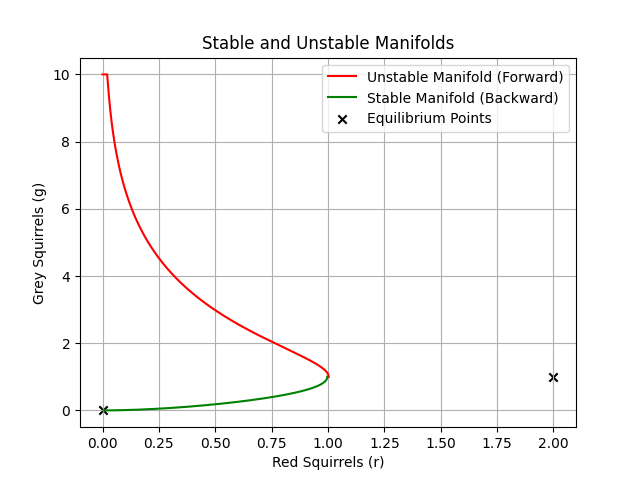
\includegraphics[scale = 0.5]{./images/stable-unstable-manifolds}
        \label{fig:stable-unstable-manifolds}
    \end{center}

\subsubsection*{Comparison of Theory vs. Numerical Estimation}

    The values we computed near the saddle align well with the theoretical eigenvector directions that we calculated earlier. However, as the values move further away from the saddle, we see more deviations caused by nonlinear effects and the numerical manifolds diverge from the linear stability prediction.

    The accuracy can be improved by using smaller time steps in our numerical estimation, but this comes with a higher cost of computational power.

    Backward time-stepping is also particularly sensitive to numerical errors; as it will amplify them over time.

    In conclusion, the numerical estimates generally agree with the theoretical linear stability analysis, especially near the saddle.


\subsection*{Nullclines and Equilibria}
    Using the extended version of the Lotka Volterra model:
    \begin{equation}
        \dot{r} = r(1 - r - g), \qquad \dot{g} = g(a - r - bg).
    \end{equation}
    \begin{center}
    a=2, b=3
    \end{center}
    we are able to find and classify the equilibrium points.
     \\Nullclines are the lines given when $\dot{r}=0$ or $\dot{g}=0$. \\The r-nullclines are found to be:
     \[r=0, \qquad 1-r-g=0\] and g-nullclines:\[g=0, \qquad 2-r-3g=0\]The equilbrium points occur when the r-nullclines intersect with the g-nullclines as seen below:
     \begin{center}
        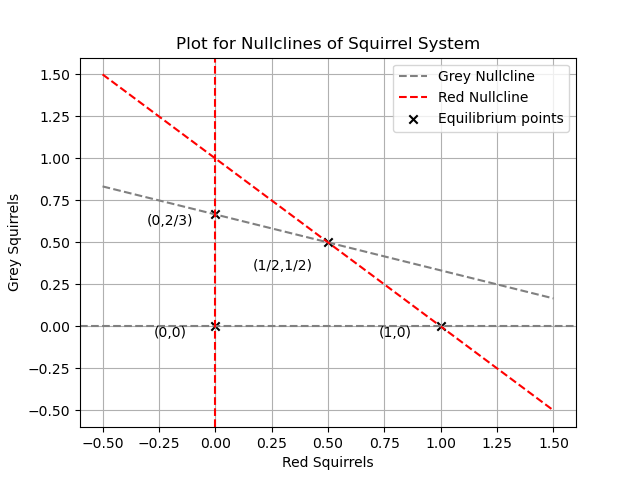
\includegraphics[scale = 0.7]{./images/nullclineplot}
    \end{center}
     Then, using eigenvalues, these points can be classified. We make a new Jacobian matrix (J)
     \[
        J = \begin{pmatrix} 1 - 2r - g & - r \\ - g & 2 - r - 3g
        \end{pmatrix}
    \]

    \[
    \lambda= \frac{-(3r+7g-3)\pm\sqrt{(3r+7g-3)^2-4(2-5r+2r^2-8g+6g^2+12rg)}}{2}
    \]


    So the eigenvalues for $(0,0)$ are:
    \[\lambda = \frac{3\pm\sqrt{1}}{2}\]
    \[\therefore \lambda = 1, \lambda = 2 \]

    Both lambda values are real and positive which means that $(0,0)$ is an improper unstable node.

    Then for $(1,0)$:
    \[\lambda = \frac{\pm\sqrt{4}}{2}\]
    \[\therefore \lambda = 1, \lambda = -1\]

    Both are real but one value is negative and the other is positive. This means that $(2,1)$ is a saddle point.

    At the point $(0,\frac{2}{3})$:
    \[\lambda = \frac{\frac{-5}{3}\pm\sqrt{\frac{49}{9}}}{2}\]
    \[\therefore \lambda =\frac{1}{3} , \lambda = -2\]
    This is also a saddle.

    At ($\frac{1}{2},\frac{1}{2}$):
    \[\lambda=-1\pm\frac{\sqrt{2}}{2}\]
    This point is a stable improper node as both eigenvalues are negative but they are not equal.
    All of these points are robust enough to be unchanged by the non-linear terms in the model.



\subsection*{Ecosystem management}
    Now we consider a situation where the parameter $b$ is decreasing due to environemntal factors. We want to find the critical value of $b$ at which there are no equilibrium points with a positive red and grey squirrel population. To do this we first look at the equation of our nullcline dependant on $a$ and $b$.
    \[
        g=\frac{a-r}b{}
    \]
    We then find the intersection of this nullcline with the one of equation $g=1-r$ in terms of $b$ and $a$ using substitution.
    \[
        r=\frac{b-a}{b-1}, g=1-\frac{b-a}{b-1}
    \]
    Next we calculate the value of $b$ where the nullclines intersect at 0 for $a=2$.
    \[
        r=\frac{b-2}{b-1}=0
    \]
    \[
        b-2=0
    \]
    \[
        b=2
    \]
    We then plotted our nullclines for $a=2$ and $b=2$
    \begin{figure}
        \centering
        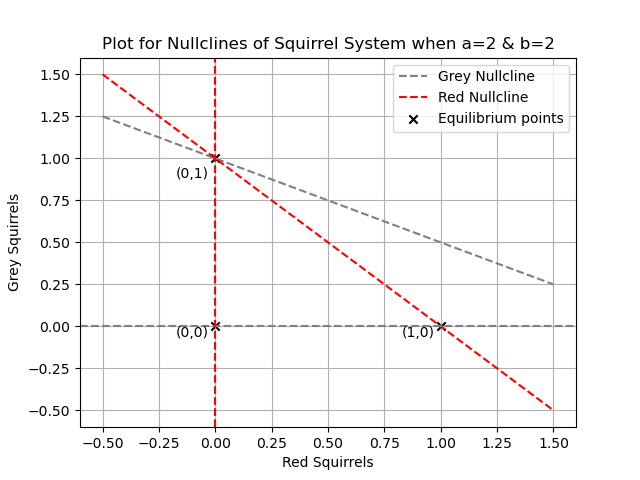
\includegraphics[scale = 0.7]{./images/nullclineplotb=2}
        \caption{Nullclines for $(2)$ with $a=2$ and $b=2$}
        \label{fig:nullclines22}
    \end{figure}
    We were then told that the ecosystem managers have the ability to change the value of parameter $a$, and were asked to find how to change $a$ in order to offset the change in $b$. To do this, we found $\dot{a}$ in terms of $\dot{b}$ when $\ddot{g}=0$. As we know where the equilibrium point is, we have the initial conditions $g=0.5,r=0.5,\dot{g}=0$
    \[
        \dot{g}=g(a-r-bg)
    \]
    \[
        \dot{g}=0.5(a-0.5-0.5b)
    \]
    \[
        \ddot{g}=0.5(\dot{a}-0.5\dot{b})=0
    \]
    \[\dot{a}-0.5\dot{b}=0\]
    \[\dot{a}=0.5\dot{b}\]
    If you decrease parameter $a$ by too much, then there ceases to be a co-existing stable equilibruim of red and grey squirrels, as the nullclines do not intersect with a positive population of red and grey squirrels. In Figure \ref{fig:nullclines52} we have used $a=0.5$ and $b=2$.
    \begin{figure}
    \centering
        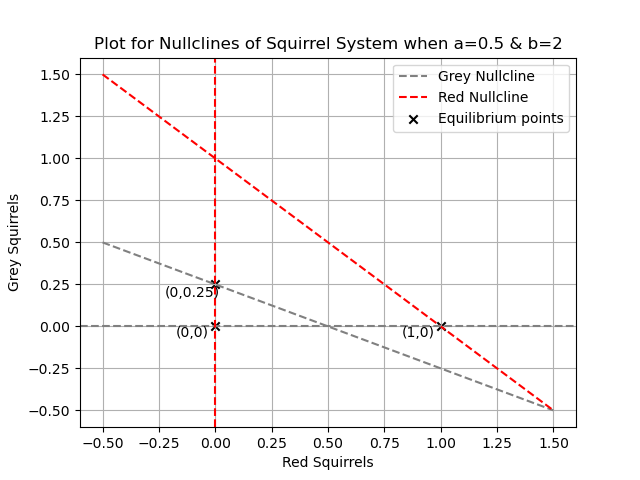
\includegraphics[scale = 0.7]{./images/nullclineplotachanged}
        \caption{Nullclines for $(2)$ with $a=0.5$ and $b=2$}
        \label{fig:nullclines52}
    \end{figure}

    As $b$ approaches 0, the gradient of the nullcline approaches $-\infty$ while its intersection approaches $\infty$, and the line of approaches $r=0$, meaning there is no way for it to intersect when the number of red and grey squirrels is positive.

\subsection*{Red and grey squirrels in the real world}

     Red squirrels are the only squirrel species that are native to the UK and have been living here for around 10,000 years. However nowadays the most common species of squirrel found in most parts of the UK is the grey squirrel. Grey squirrels were introduced to the Uk from North America by the Victorians$_{2}$ in the 1870s and they carry a parapoxvirus which is a disease that does not appear to affect the health of the grey squirrels, but kills red squirrels when passed onto them. Additionally, grey squirrels are more likely to eat green acorns, which means they were eating the food before red squirrels were able to. This significantly decreased the amount of food available for the red squirrels causing them to be put under pressure which prevented them from breeding and having a sufficient amount of food to keep them alive. As a result of this the red squirrel population has dropped from around 3.5 million to 140,000 since the introduction of grey squirrels$_{1}$. However, there are other factors that may have contributed to the decline in the red squirrel population. For example, the loss of habitat due to the decline in the coverage of woodlands as urbanization has advanced, this causes a loss of food and safe living environments for the squirrels. Similarly, road traffic and predators are also significant factors that would have contributed to the decline in population of red squirrels. Additionally, natural environments are not static and many changes in conditions could have contributed to the decline including change of temperature and PH, however environments are often changing and species tend to adapt to those changes as they happen, whereas the red squirrels were not given this chance due to the invasive nature of the grey squirrels$_{3}$. Because of this it is difficult to predict what effect the other possible factors would've had if it wasn't for the introduction of grey squirrels, making grey squirrels the major contributor to the decline in the population of red squirrels.

     There are some places in the UK that grey squirrels are unable to access such as islands due to the fact that they can't swim far enough. Some examples include the Isle of Wight and Brownsea, also Anglesey has recently been declared free of grey squirrels$_{4}$. Therefore the population of red squirrels on these islands is not affected by the grey squirrels - essentially staying constant - so we shouldn't keep decreasing the population size as suggested by the model. Instead we should consider adding a constant value that represents the total population on all the islands (around 4000 red squirrels)$_{5}$,$_{6}$,$_{7}$ and this should be included in the extended Lotka-Volterra model.

     Additionally, grey squirrels are hunted in certain areas as they are considered vermin. This could have an impact on the population of grey squirrels that isn't considered in the model. Hence, another term dependent on the population of grey squirrels should be added to the extended Lotka-Volterra model: as the population size increases, more squirrels are going to be hunted due to the larger population density, which will decrease the population again.

     \scriptsize{$_{1}$Woodland Trust: Red Squirrel Facts. Retrieved March 2025 from \\ https://www.woodlandtrust.org.uk/blog/2018/11/red-squirrel-facts/ \\ $_{2}$Wildlife Trusts: Red squrrels. Retrieved March 2025 from https://www.wildlifetrusts.org/saving-species/red-squirrels \\ $_{3}$Roberts, M.G., Heesterbeek, J.A.P., 2001. Infection dynamics in ecosystems: on the interaction between red and grey squirrels, pox virus, pine martens and trees. J. Roy. Soc. Interface, 18, 20210551. https://doi.org/10.1098/rsif.2021.0551 \\ $_{4}$The place that has wiped out grey squirrels (2015) BBC News. \\ Available at: https://www.bbc.co.uk/news/magazine-34603394 (Accessed: March 2025). \\ $_{5}$Red Squirrels and wildlife on the Isle of Wight, Visit Isle Of Wight. \\ Available at: https://www.visitisleofwight.co.uk/things-to-do/activities/wildlife \\ (Accessed: March 2025). \\ $_{6}$Brownsea Island (2025) Dorset Wildlife Trust. \\ Available at: https://www.dorsetwildlifetrust.org.uk/brownsea-island (Accessed: March 2025). \\  $_{7}$Visit Anglesey, Red Squirrels Available at: https://angleseyisle.co.uk/red-squirrels (Accessed: March 2025).}



     \textbf{}

     \lstinputlisting[language=Python,label={lst:lstinputlisting}]{./main.py}
\end{document}